%%
%% This is file `sample-sigconf-authordraft.tex',
%% generated with the docstrip utility.
%%
%% The original source files were:
%%
%% samples.dtx  (with options: `all,proceedings,bibtex,authordraft')
%% 
%% IMPORTANT NOTICE:
%% 
%% For the copyright see the source file.
%% 
%% Any modified versions of this file must be renamed
%% with new filenames distinct from sample-sigconf-authordraft.tex.
%% 
%% For distribution of the original source see the terms
%% for copying and modification in the file samples.dtx.
%% 
%% This generated file may be distributed as long as the
%% original source files, as listed above, are part of the
%% same distribution. (The sources need not necessarily be
%% in the same archive or directory.)
%%
%%
%% Commands for TeXCount
%TC:macro \cite [option:text,text]
%TC:macro \citep [option:text,text]
%TC:macro \citet [option:text,text]
%TC:envir table 0 1
%TC:envir table* 0 1
%TC:envir tabular [ignore] word
%TC:envir displaymath 0 word
%TC:envir math 0 word
%TC:envir comment 0 0
%%
%% The first command in your LaTeX source must be the \documentclass
%% command.
%%
%% For submission and review of your manuscript please change the
%% command to \documentclass[manuscript, screen, review]{acmart}.
%%
%% When submitting camera ready or to TAPS, please change the command
%% to \documentclass[sigconf]{acmart} or whichever template is required
%% for your publication.
%%
%%
\usepackage{makecell}
\usepackage{float}
\documentclass[sigconf]{acmart}
%%
%% \BibTeX command to typeset BibTeX logo in the docs
\AtBeginDocument{%
  \providecommand\BibTeX{{%
    Bib\TeX}}}

%% Rights management information.  This information is sent to you
%% when you complete the rights form.  These commands have SAMPLE
%% values in them; it is your responsibility as an author to replace
%% the commands and values with those provided to you when you
%% complete the rights form.
% \setcopyright{acmlicensed}
% \copyrightyear{2018}
% \acmYear{2018}
% \acmDOI{XXXXXXX.XXXXXXX}
% %% These commands are for a PROCEEDINGS abstract or paper.
\acmConference[World Wide Web Conference 2026]{Make sure to enter the correct
  conference title from your rights confirmation email}{April 13--17,
  2026}{Dubai, United Arab Emirates}
%%
%%  Uncomment \acmBooktitle if the title of the proceedings is different
%%  from ``Proceedings of ...''!
%%
%%\acmBooktitle{Woodstock '18: ACM Symposium on Neural Gaze Detection,
%%  June 03--05, 2018, Woodstock, NY}
% \acmISBN{978-1-4503-XXXX-X/2018/06}


%%
%% Submission ID.
%% Use this when submitting an article to a sponsored event. You'll
%% receive a unique submission ID from the organizers
%% of the event, and this ID should be used as the parameter to this command.
%%\acmSubmissionID{123-A56-BU3}

%%
%% For managing citations, it is recommended to use bibliography
%% files in BibTeX format.
%%
%% You can then either use BibTeX with the ACM-Reference-Format style,
%% or BibLaTeX with the acmnumeric or acmauthoryear sytles, that include
%% support for advanced citation of software artefact from the
%% biblatex-software package, also separately available on CTAN.
%%
%% Look at the sample-*-biblatex.tex files for templates showcasing
%% the biblatex styles.
%%

%%
%% The majority of ACM publications use numbered citations and
%% references.  The command \citestyle{authoryear} switches to the
%% "author year" style.
%%
%% If you are preparing content for an event
%% sponsored by ACM SIGGRAPH, you must use the "author year" style of
%% citations and references.
%% Uncommenting
%% the next command will enable that style.
%%\citestyle{acmauthoryear}

\usepackage{amsmath,amssymb}
\usepackage{booktabs}
\usepackage{microtype}
\usepackage{graphicx}
\usepackage{xcolor}
\usepackage{tikz}
\usetikzlibrary{positioning,arrows.meta}

\settopmatter{printacmref=false,printfolios=true}
\renewcommand\footnotetextcopyrightpermission[1]{}
%%
%% end of the preamble, start of the body of the document source.
\begin{document}

%%
%% The "title" command has an optional parameter,
%% allowing the author to define a "short title" to be used in page headers.
\title{LeTCC-ZK: Smooth, Verifiable Distributed Inference via Spline-Coded Computing}

%%
%% The "author" command and its associated commands are used to define
%% the authors and their affiliations.
%% Of note is the shared affiliation of the first two authors, and the
%% "authornote" and "authornotemark" commands
%% used to denote shared contribution to the research.


\author{Ekaterina Pavlova}
\affiliation{
  \institution{Skolkovo Institute of Science and Technology}
  \city{Moscow}
  \country{Russia}
}
\email{ekaterina.pavlova@skoltech.ru}

% --- Supervisor / Advisor (placeholder) ---
\author{Alexey Frolov}
\authornote{Supervisor/Advisor.}
\affiliation{
  \institution{Skolkovo Institute of Science and Technology}
  \city{Moscow}
  \country{Russia}
}
\email{Al.Frolov@skoltech.ru}


\renewcommand{\shortauthors}{Pavlova E.}

%%
%% The abstract is a short summary of the work to be presented in the
%% article.
\begin{abstract}
Web-facing inference networks---federated clusters, oracle committees, and market-data aggregation fabrics---must deliver accurate predictions despite stragglers and Byzantine workers.
Classical threshold-coded computing (e.g., MDS/Lagrange codes) offers exact recovery only while a fixed response quorum is met; once availability drops below that threshold, decoding becomes ill-posed and accuracy can collapse abruptly.
This paper outlines my dissertation direction on smoothly degrading and cryptographically verifiable distributed inference.

I propose LeTCC-ZK, an end-to-end redundancy layer that (i) encodes each input into $N$ redundant shards along a learned one-dimensional parameterization, (ii) requires each worker to return its shard output together with a per-shard zk-SNARK proof of correct execution, (iii) verifies and filters outputs before aggregation, and (iv) decodes at a fixed interior anchor via natural cubic-spline interpolation.
If the composed function $g=f\circ\gamma$ is $C^4$ along the learned curve $\gamma$, spline interpolation yields reconstruction error $O(h^4)$ where $h$ is the fill distance of the verified knots, inducing non-threshold (graceful) degradation as shards disappear.
LeTCC-ZK also outputs a calibrated reliability score that downstream services (e.g., smart contracts or web APIs) can consume to make risk-aware decisions.
\end{abstract}


\keywords{Coded computing, verifiable computation, zero-knowledge proofs, Byzantine robustness, federated inference, blockchain oracles}

\maketitle

\section{Introduction}
Distributed inference is becoming a standard component of web and web-adjacent systems, where predictions must be produced under heterogeneous latency, partial participation, and limited trust. In federated deployments, inference and/or training-time evaluation is executed across large populations of edge devices to reduce data movement and preserve user privacy; production FL systems have been deployed at scale, and keyboard language modeling is a canonical example of this paradigm \cite{mcmahan2017fedavg,bonawitz2019scale,hard2018keyboard}. In decentralized applications, oracle committees and decentralized oracle networks provide externally sourced signals---most prominently price feeds---that smart contracts consume to trigger liquidations, settlements, and other state transitions; Chainlink is a widely deployed reference architecture for such oracle networks \cite{ellis2017chainlink,breidenbach2021chainlink2}. In financial and sensing infrastructures, aggregation fabrics consolidate multiple feeds into a single downstream-consumable view; in U.S. equities, the Securities Information Processor (SIP) is a concrete, operational instance of market-data consolidation \cite{ctaSIP}. Across these settings, the system objective is not merely to compute a prediction, but to do so continuously and defensibly as participation fluctuates.

Two operational realities complicate this objective. First, web-scale participation is bursty: devices disconnect, validators miss rounds, and compute availability varies widely, creating stragglers and erasures that can remove a large fraction of contributions within a single latency budget. This has motivated a long line of straggler-mitigation techniques in distributed ML, including redundancy and coding-based approaches \cite{karakus2017straggler}. Second, contributors may be adversarial rather than merely slow: federated participants can submit model-poisoning or backdoored updates, and oracle providers can attempt to bias aggregates when incentives favor manipulation \cite{bagdasaryan2020backdoor,nadler2025oracles}. For web services that sit on critical decision paths (e.g., automated moderation, ranking, fraud signals, or on-chain risk engines), a single incorrect contribution can be more damaging than a missing one.

Accordingly, many deployments require continuous service under uncertainty: the system should return an output even when only a subset of workers respond, it should prevent Byzantine contributions from influencing the result, and it should quantify residual risk so downstream components can choose conservative actions when reliability is low. These requirements are poorly matched by threshold-based recovery mechanisms that exhibit an all-or-nothing “cliff” once responses fall below a fixed quorum. This dissertation therefore targets distributed inference layers that degrade smoothly under shard loss, filter incorrect contributions with cryptographic assurance, and expose an explicit reliability signal to web and decentralized consumers.

\section{Problem Statement}
We consider inference of a fixed model $f:\mathbb{R}^{d_x}\!\to\!\mathbb{R}^{d_y}$ using $N$ workers under stragglers and Byzantine behavior.
Given an input $x$, an encoder produces $N$ shard inputs $(u_1,\dots,u_N)$; worker $i$ returns an output $y_i$.
The aggregator must produce an estimate $\hat y$ of the uncoded output $y=f(x)$ using only the subset of outputs that arrive in time and are deemed valid.

\paragraph{P1: Threshold brittleness.}
MDS and polynomial/Lagrange schemes reconstruct exactly only if the number of responses exceeds a fixed threshold; below it decoding fails or becomes ill-conditioned, yielding an abrupt cliff in accuracy \cite{yu2019lagrange}.

\paragraph{P2: Byzantine influence.}
If workers may return arbitrary outputs, incorrect shards can bias reconstruction unless additional defences are used.
Robust decoding alone is often insufficient in adaptive adversarial environments; per-shard verification is preferable when feasible \cite{tang2021avcc}.

\paragraph{P3: Missing reliability interface.}
Downstream web systems (e.g., smart contracts, alerting pipelines, automated decisioning) require an explicit reliability signal reflecting both model uncertainty and system uncertainty (availability and verification outcomes).

\paragraph{Objective.}
Design a distributed inference layer that:
(i) produces a meaningful output for any verified subset size $H$ (no hard failure point),
(ii) prevents Byzantine shards from affecting the aggregate except with negligible probability, and
(iii) exposes a calibrated reliability score for risk-aware downstream use.



\begin{figure}[t]
\centering
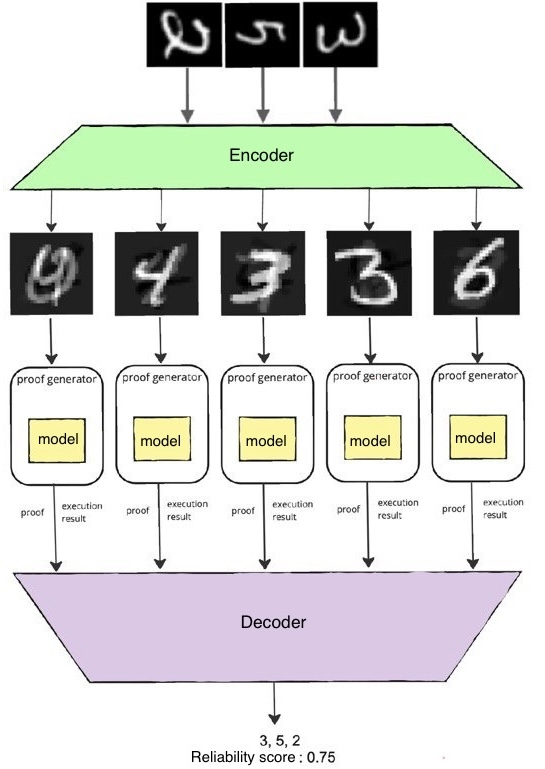
\includegraphics[width=0.7\linewidth]{img/ai (6).png}
\caption{System overview. The encoder produces redundant shards; workers return outputs with per-shard proof generation; the decoder reconstructs the prediction and outputs a reliability score.}
\label{fig:overview}
\end{figure}


\section{State of the Art}
Threshold-coded computing is the classical approach for straggler mitigation in distributed computation. In particular, Lagrange Coded Computing (LCC) and related polynomial/MDS constructions provide exact recovery together with strong resiliency and, in some settings, privacy guarantees, but only as long as the aggregator receives a sufficient number of responses \cite{yu2019lagrange}. Once availability falls below this hard threshold, decoding becomes ill-posed and performance can collapse, which is a poor fit for web-scale deployments where participation is frequently bursty and unpredictable.

To address this brittleness, approximate and smooth coded computing methods have emerged. Learning-Theoretic Coded Computing (LeTCC) trains encoder and decoder maps end-to-end and empirically exhibits graceful degradation as fewer worker outputs are available \cite{moradi2024letcc}. In a similar spirit, BACC-style schemes move beyond polynomial assumptions by using alternative interpolation mechanisms designed to better handle non-polynomial workloads \cite{jahani2020bacc}. While these lines of work reduce the threshold cliff, they typically do not provide cryptographically strong correctness guarantees against Byzantine workers, leaving the reconstruction vulnerable when malicious outputs are included.



A complementary thread studies adversarial and verifiable coded computing. General adversarial coded computing develops models and limits for Byzantine settings, characterizing when and how adversarial behavior can bias reconstruction \cite{moradi2025adversarial}. Adaptive Verifiable Coded Computing (AVCC) incorporates verification ideas to mitigate malicious behavior \cite{tang2021avcc}. However, existing verifiable designs commonly remain coupled to meeting a reconstruction condition (or an effective threshold) for correctness and do not directly provide a non-threshold, smoothly degrading inference mechanism.

Zero-knowledge proofs provide a distinct, cryptographic route to correctness. Succinct zk-SNARKs such as Groth16 enable efficient verification of correct computation while hiding private inputs and internal witness data \cite{groth2016}. Although zkML tooling is improving and makes proof-carrying inference increasingly feasible, per-shard zk verification has not yet been systematically combined with a smooth redundancy and decoding mechanism that is explicitly designed to degrade gracefully under missingness.

The resulting gap is an end-to-end design that simultaneously eliminates the threshold cliff through smooth decoding, filters Byzantine shards cryptographically at per-shard granularity, and exposes an actionable reliability score that downstream web systems can consume for risk-aware operation.



\section{Proposed Approach}
I propose LeTCC-ZK, a redundancy and verification layer inserted between the base model $f$ and a distributed worker pool (fig.~\ref{fig:overview}).

% \subsection{Pipeline}
LeTCC-ZK executes five stages: encode $\to$ compute $\to$ prove $\to$ verify $\to$ decode which is shown on fig.~\ref{fig:pipeline}.


\begin{table}[H]
\caption{High-level comparison of coded-inference schemes}
\label{tab:feature-matrix}
\centering\small
\begin{tabular}{lccc}
\toprule
Method & \shortstack{Smooth\\degr.} & Verifiable & Notes \\
\midrule
MDS / RS & \texttimes & \texttimes & exact if threshold met \\
LCC \cite{yu2019lagrange} & \texttimes & \texttimes & polynomial assumption \\
BACC \cite{jahani2020bacc} & $\sim$ & \texttimes & approximate interpolation \\
AVCC \cite{tang2021avcc} & \texttimes & \checkmark & verifiable but thresholded \\
\textbf{LeTCC-ZK (ours)} & \checkmark & \checkmark & spline-coded + per-shard zk \\
\bottomrule
\end{tabular}
\end{table}


\subsection{Decoding via Splines}
The encoder learns a one-dimensional parameterization $\gamma:[0,1]\to\mathbb{R}^{d_x}$ and knot locations $\beta_i\in[0,1]$.
Each worker receives $u_i=\gamma(\beta_i)$ and returns $y_i=f(u_i)$, i.e., samples of $g(t)=f(\gamma(t))$.
The decoder reconstructs the target output at a fixed interior anchor $t_\star\in(0,1)$ (e.g., $t_\star=\tfrac12$) using the natural cubic spline interpolant $\hat g$ built from the verified knot set.

Let $\beta_{(1)}<\cdots<\beta_{(H)}$ be the surviving verified knots and define fill distance
\[
h = \max\!\Bigl\{\beta_{(1)}-0,\ \max_{k=1}^{H-1}(\beta_{(k+1)}-\beta_{(k)}),\ 1-\beta_{(H)}\Bigr\}.
\]



\begin{figure*}[]
\centering
\resizebox{0.92\linewidth}{!}{%
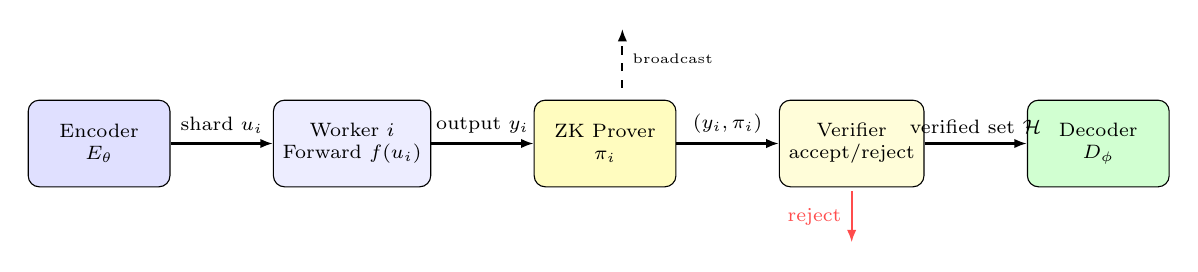
\begin{tikzpicture}[
    node/.style={
      draw,rounded corners,align=center,
      font=\scriptsize,
      minimum height=1.1cm,minimum width=1.8cm},
    arr/.style={-{Latex[length=1.6mm]},thick},
    >=Latex
]
\node[node,fill=blue!12]                         (enc)  {Encoder\\$E_\theta$};
\node[node,fill=blue!7 ,right=1.3cm of enc]      (wrk)  {Worker $i$\\Forward $f(u_i)$};
\node[node,fill=yellow!25,right=1.3cm of wrk]    (prov) {ZK Prover\\$\pi_i$};
\node[node,fill=yellow!15,right=1.3cm of prov]   (ver)  {Verifier\\accept/reject};
\node[node,fill=green!18 ,right=1.3cm of ver]    (dec)  {Decoder\\$D_\phi$};

\draw[arr] (enc)  -- node[above]{\scriptsize shard $u_i$}(wrk);
\draw[arr] (wrk)  -- node[above]{\scriptsize output $y_i$}(prov);
\draw[arr] (prov) -- node[above]{\scriptsize $(y_i,\pi_i)$}(ver);
\draw[arr] (ver)  -- node[above]{\scriptsize verified set $\mathcal{H}$}(dec);

\draw[arr,red!70] (ver.south)++(0,-0.05) -- ++(0,-0.65)
      node[midway,left]{\scriptsize reject};

\draw[arr,dashed] (prov.north) ++(0.22,0.15) -- ++(0,0.75)
      node[midway,right]{\tiny broadcast};
\end{tikzpicture}}
\caption{LeTCC-ZK encode--prove--verify--decode workflow. Invalid proofs are rejected; only verified outputs reach the spline decoder.}
\label{fig:pipeline}
\end{figure*}

\begin{figure}[H]
  \centering
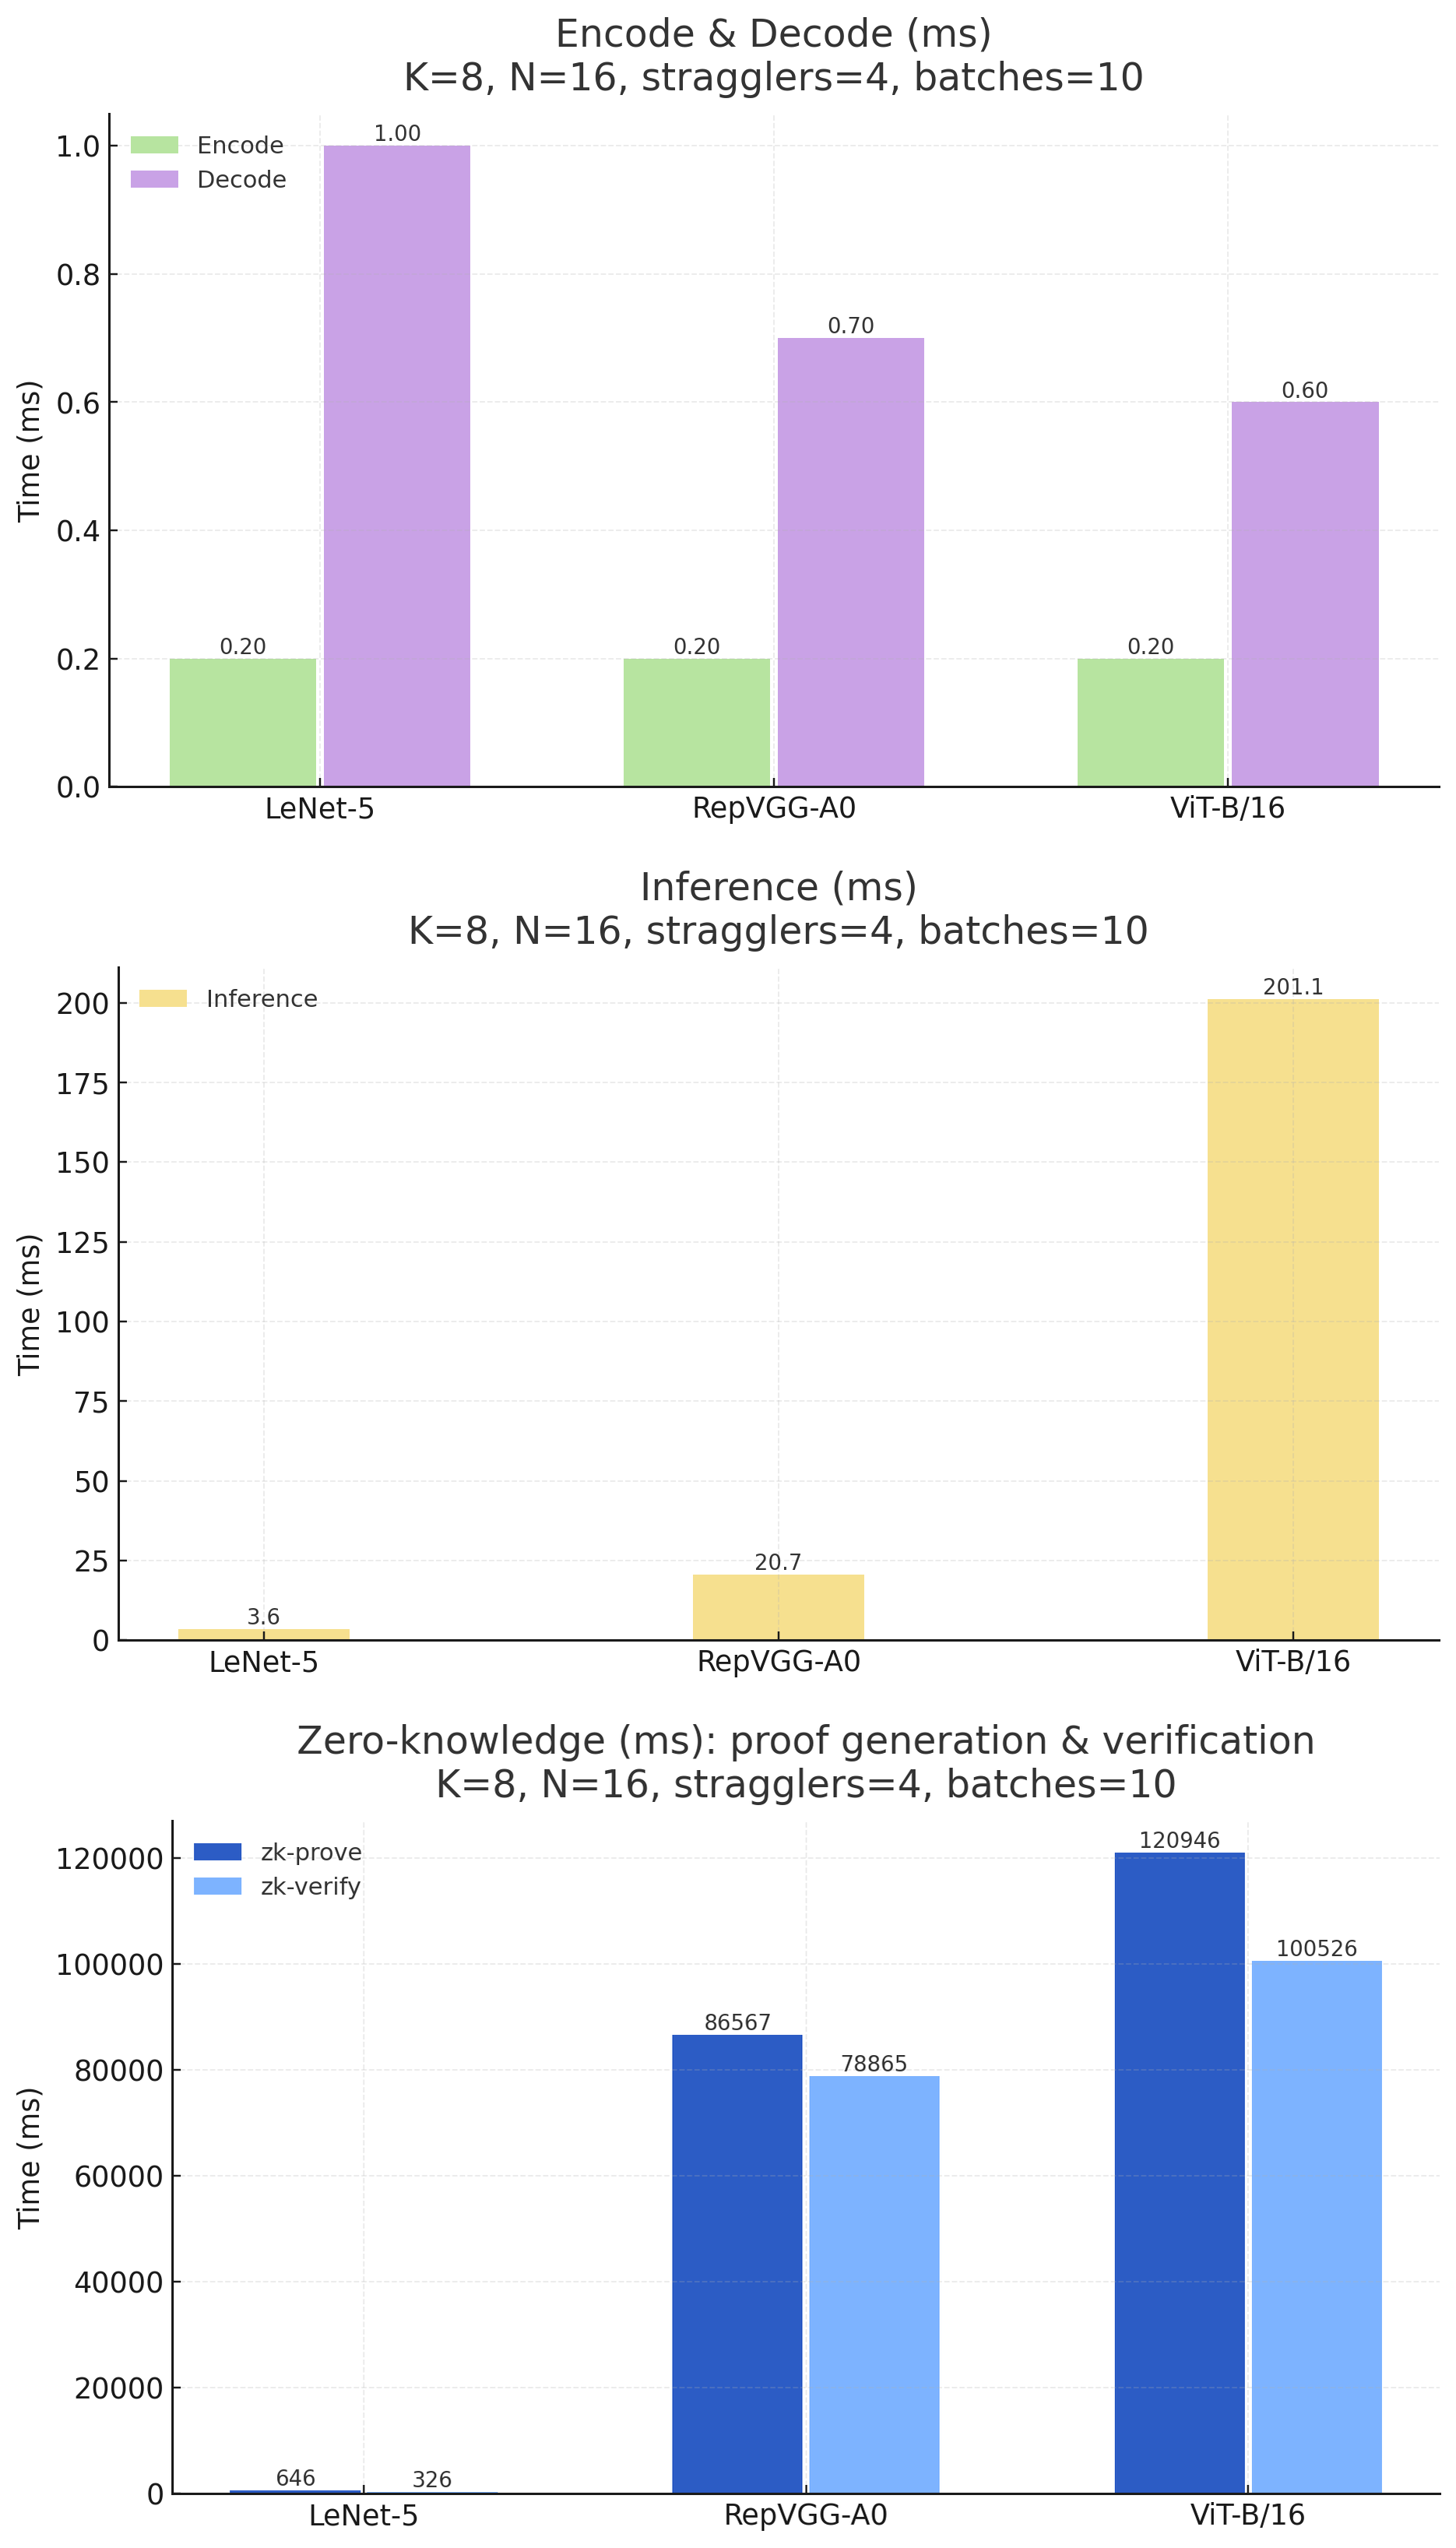
\includegraphics[width=0.99\linewidth]{img/timings_combined_3panels_horizontal_palette_v2 (1).png}
  \caption{Runtime breakdown: encoding/decoding overhead, inference time, and zero-knowledge proof generation/verification.}
  \label{fig:acc}
\end{figure}

If $g\in C^4([0,1])$, then $\|g-\hat g\|_\infty=O(h^4)$, implying pointwise reconstruction error
$\|g(t_\star)-\hat g(t_\star)\|_2=O(h^4)$ \cite{deboor2001,hall1976}.
Thus accuracy degrades continuously as $h$ increases (no hard threshold).








\subsection{Byzantine Filtering via zk-SNARKs}
Each worker submits $(y_i,\pi_i)$ where $\pi_i$ is a zk-SNARK proof (e.g., Groth16 \cite{groth2016}) attesting $y_i=f(u_i)$.





The statement binds a round identifier $r$, shard index $i$, a commitment $C$ to shard inputs (or openings), and a model identifier (\texttt{modelHash}).




The aggregator verifies $\pi_i$ and discards invalid shards prior to decoding.





If the admission policy limits verification attempts to at most $s$ per round, the probability that any invalid shard is accepted is at most $s\cdot\mu(\kappa)$ (union bound), where $\mu(\kappa)$ is the negligible soundness error.





\section{Methodology}
\subsection{Training the Redundancy Layer}
We train $(E_\theta,D_\phi)$ offline with the base model $f$ fixed.
For each training sample $x$, we generate shards via $\gamma(\beta_i)$ and simulate missingness by sampling subsets $\mathcal{H}$ under fault models (independent thinning and clustered loss).
We minimize reconstruction error:
\[
\mathcal{L}_{\text{recon}}=\mathbb{E}_{x,\mathcal{H}}\bigl[\|f(x)-D_\phi(\{(\beta_i,f(\gamma(\beta_i)))\}_{i\in\mathcal{H}})\|_2^2\bigr].
\]
To stabilize interpolation, we regularize knot placement to enforce (i) bracketing of $t_\star$ and (ii) bounded mesh ratio (quasi-uniform spacing), improving worst-case $h$ under loss.

\subsection{Verification and Admission Policy}
To make cryptographic filtering operational, the aggregator:
(i) enforces identical round headers $(C,r,\texttt{modelHash})$,
(ii) enforces unique indices $i$ per round,
(iii) rate-limits verification attempts to at most $s$ per round.
Only then are proofs sent to the pairing-based verifier.

\subsection{Evaluation Protocol}
We evaluate:
(1) reconstruction error vs.\ fill distance $h$ and subset fraction $H/N$,
(2) downstream accuracy vs.\ missing fraction $1-H/N$,
(3) proof verification throughput and end-to-end latency,
(4) reliability score calibration (ECE/Brier) and selective prediction curves.
Baselines include LCC \cite{yu2019lagrange}, BACC \cite{jahani2020bacc}, and AVCC \cite{tang2021avcc}, shown in table~\ref{tab:feature-matrix}.




\section{Preliminary Results}
I implemented an end-to-end prototype of the encode--prove--verify--decode pipeline to validate two claims: (i) decoding degrades smoothly as the verified subset shrinks, and (ii) overheads decompose into a lightweight redundancy layer and a heavier proof layer.



The current microbenchmark (fig.~\ref{fig:accuracy-curve},~\ref{fig:acc}) uses Apple Silicon with 48\,GB RAM, micro-batch size $K{=}8$, $N{=}16$ workers with 4 simulated stragglers, and 10 batches. I evaluated LeNet-5, RepVGG-A0, and ViT-B/16. Under increasing missing/Byzantine fractions, the spline-coded decoder exhibits continuous accuracy decline rather than a hard collapse, consistent with the qualitative behavior in the poster’s accuracy curve (smooth degradation for LeTCC-ZK versus a threshold cliff for RS/LCC).

Encoding and spline decoding are inexpensive relative to base inference: encoding is approximately 0.20\,ms per batch across models, while decoding remains 0.60--1.00\,ms. Base inference ranges from 3.6\,ms (LeNet-5) to 201.1\,ms (ViT-B/16). In the current implementation, zk proving dominates runtime (roughly 0.65\,s for LeNet-5 and $\sim$86--121\,s for RepVGG-A0/ViT-B/16), while verification is cheaper and parallelizable (roughly 0.33\,s and $\sim$79--101\,s, respectively).

Overall, these results indicate that the spline redundancy is not the bottleneck; proof generation is. This motivates dissertation work on reducing prover cost (batching/recursion or alternative proof systems) and exploiting pipeline parallelism. I also implemented a preliminary calibrator $\mathrm{Calib}(\cdot)$ trained on fault-injected runs; incorporating $H/N$ improves correspondence between confidence and label stability under shard loss.


\begin{figure}[H]
\centering
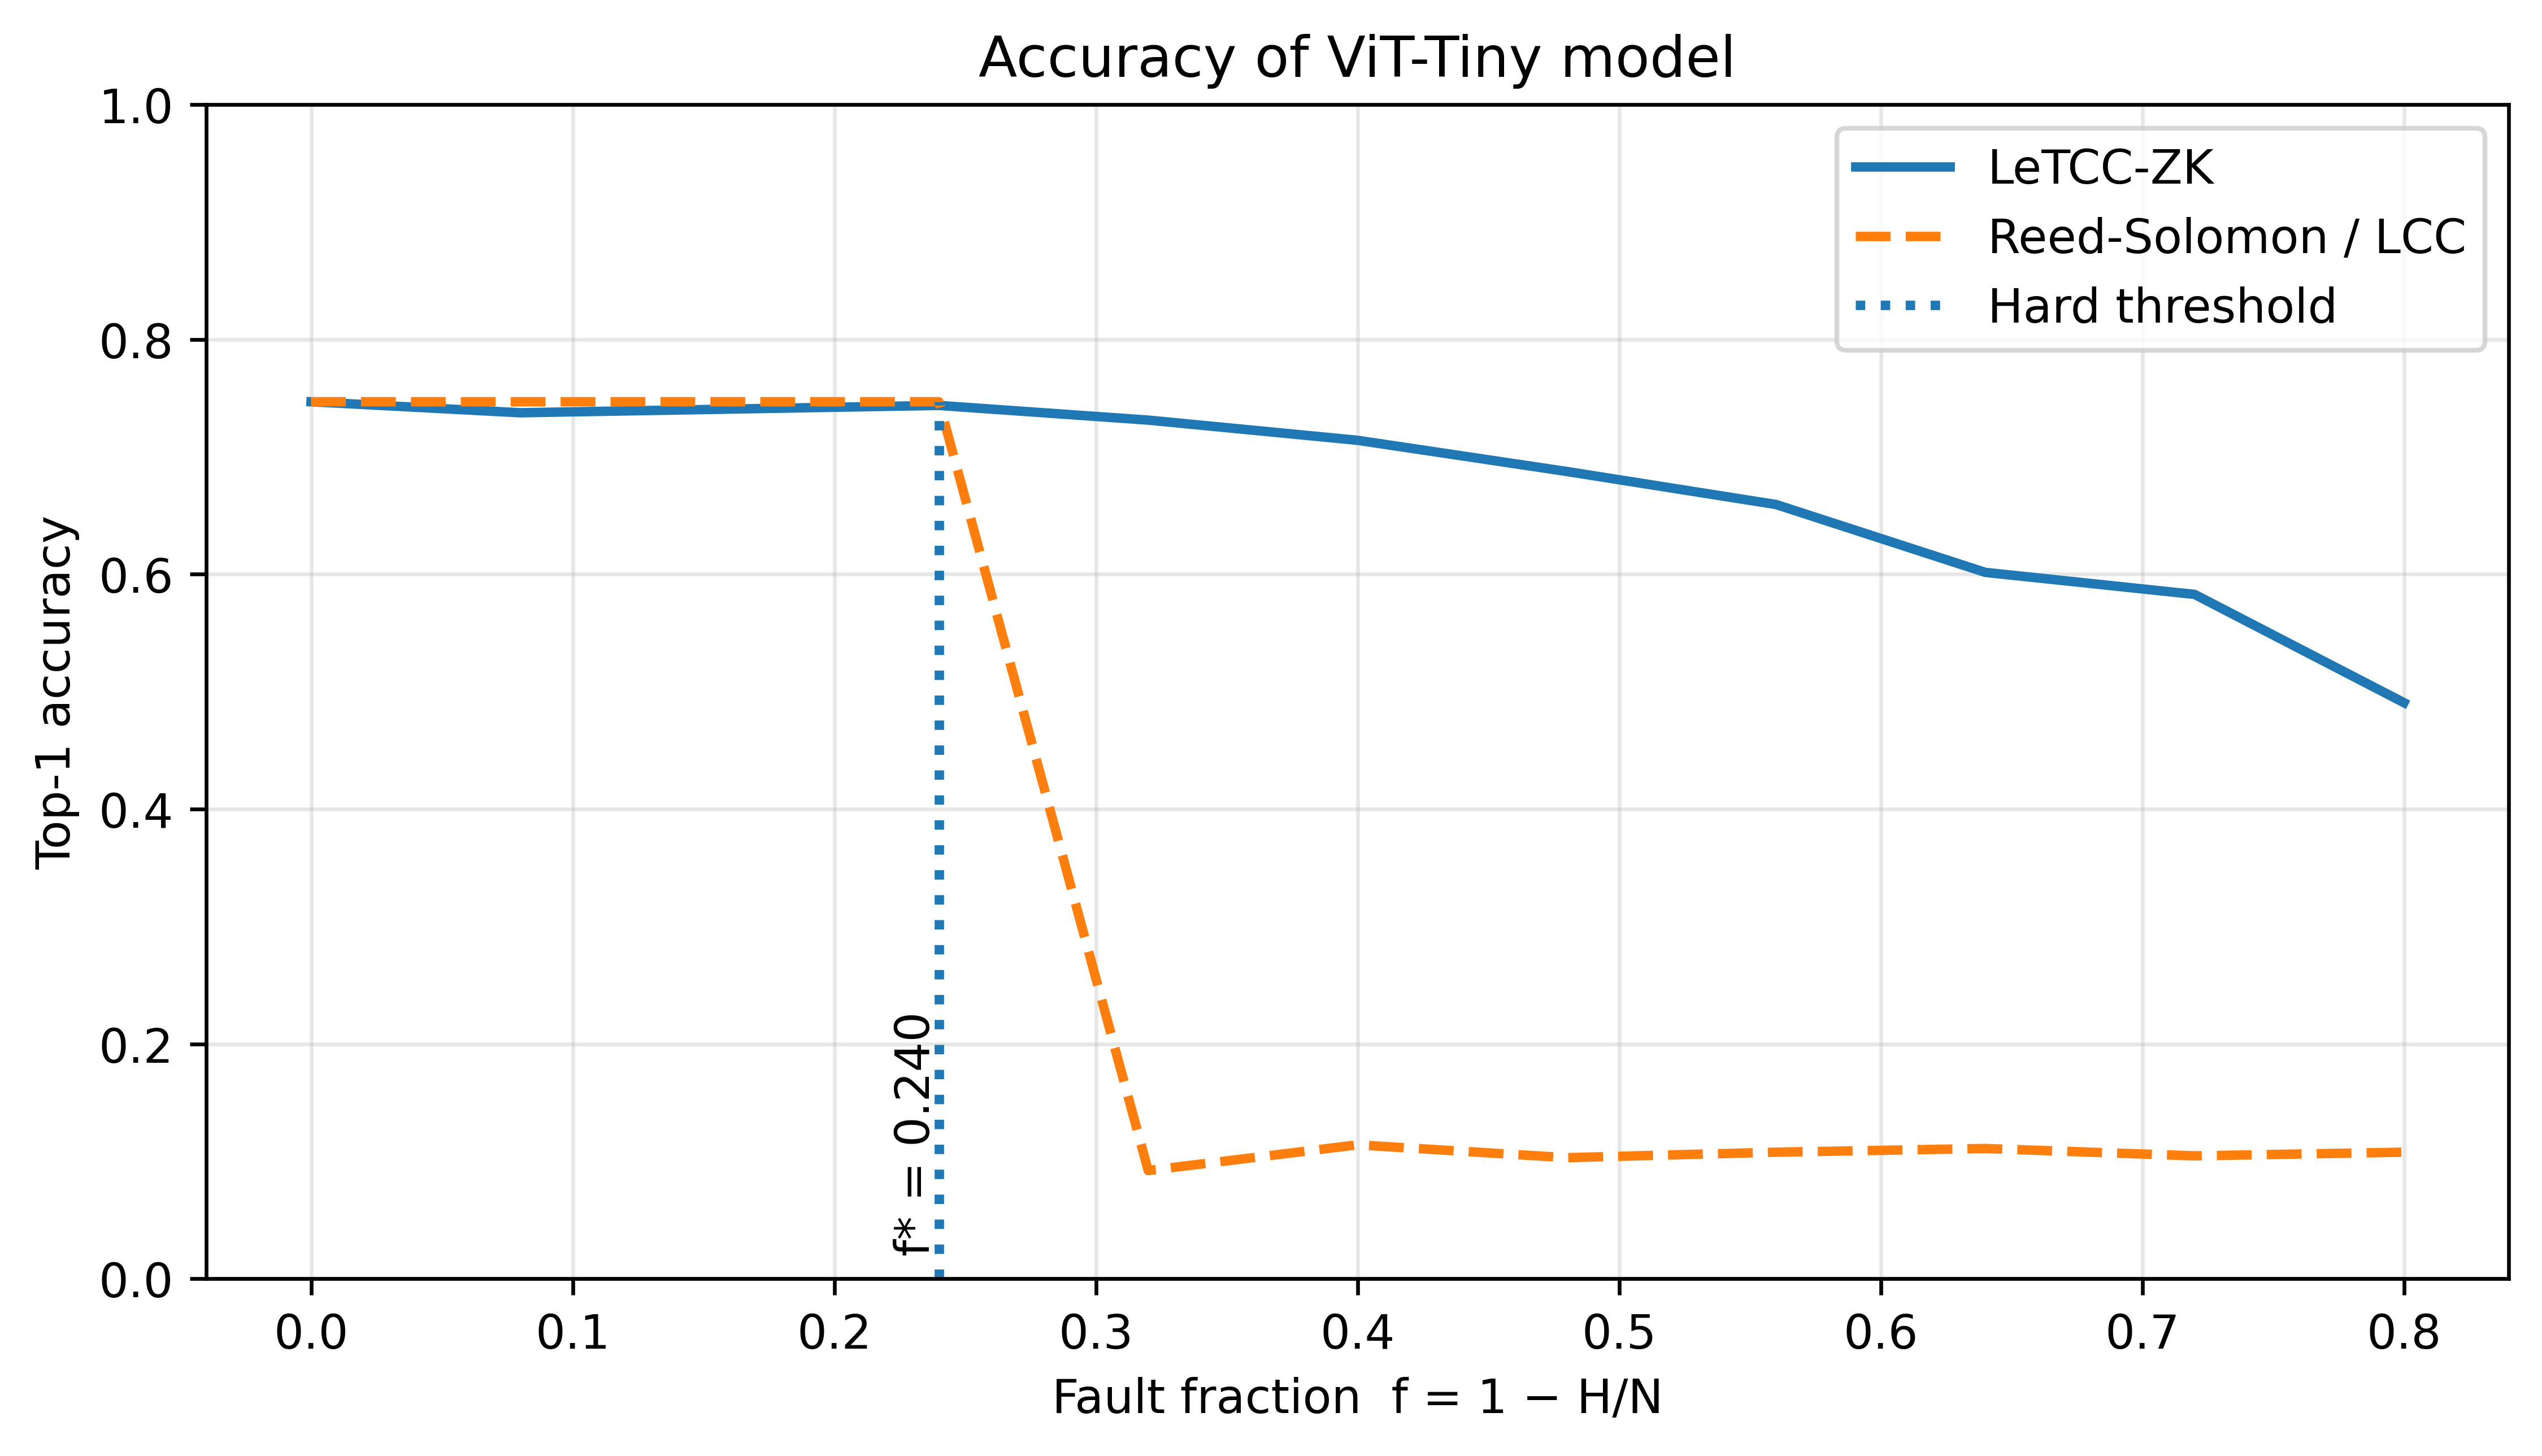
\includegraphics[width=0.99\linewidth]{img/fig1 (1) (1).jpg}
\caption{Top-1 accuracy vs.\ missing/Byzantine fraction. Smooth degradation for LeTCC-ZK vs.\ RS/LCC threshold cliff.}
\label{fig:accuracy-curve}
\end{figure}












\section{Conclusions}
LeTCC-ZK is a dissertation direction toward a web-relevant distributed inference layer that removes the threshold cliff and provides strong correctness guarantees under Byzantine workers.
Its key mechanism is spline-coded, non-threshold decoding with $O(h^4)$ reconstruction error under standard smoothness assumptions \cite{deboor2001,hall1976}, combined with per-shard zk-SNARK filtering \cite{groth2016}.
The resulting interface produces both an output $\hat y$ and an explicit reliability score $R$ for downstream risk-aware consumption.

% =========================================================
\section{Future Work}
My next steps focus on:
(i) tightening theoretical guarantees under realistic loss models (random thinning, bursty/clustered loss) and characterizing conditions on learned knots that keep mesh ratio bounded;
(ii) reducing prover cost via batching/aggregation/recursion and evaluating Plonkish/Halo2 alternatives to Groth16;
(iii) strengthening the reliability interface via broader calibration (ECE/Brier, selective prediction) and demonstrating end-to-end impact in relevant deployments such as oracle committees and federated inference gateways.


\bibliographystyle{unsrt}
\bibliography{refs}





\end{document}
\endinput
